\documentclass[../main.tex]{subfiles}

\begin{document}
\begin{example}[]
  The derivative of a function \(f(x)\) is sketched below. Suppose \(f(2) = 1\). Find the \(y\)-intercept of the line tangent to the curve \(y = f(x)\) at \(x = 2\).

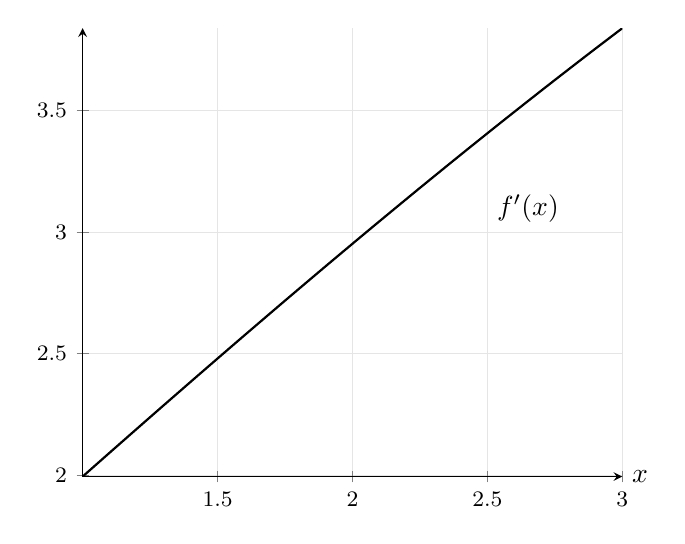
\begin{tikzpicture}
      \begin{axis}[
        axis lines = middle, % boxed, middle
        % axis equal image,
        % enlargelimits=true,
        xlabel={\(x\)}, xlabel style={anchor=west},
        % ylabel={\(y\)}, ylabel style={anchor=south},
        label style={at={(ticklabel* cs:1)}},
        ticklabel style={font=\footnotesize},
        grid=major, grid style={gray!20}, 
        smooth, samples=100, no markers,
        ]
        \addplot[thick, domain=1:3] {x*cos(x*2*pi) + 1};
        \node[above right] at (axis cs:2.5,3) {\(f'(x)\)};
      \end{axis}
    \end{tikzpicture}
\end{example}
\end{document}
